\documentclass{article}
\usepackage[utf8]{inputenc}
\usepackage{tikz}
\usetikzlibrary{shapes,arrows}
\usepackage[ruled,vlined]{algorithm2e}
\usepackage{algpseudocode}
\usepackage{multicol}
\renewcommand{\contentsname}{{\Huge Table de Matières}}
\usepackage{titlesec}
\usepackage{xcolor}
\usepackage{listings}
\usepackage{graphicx}
\usepackage[normalem]{ulem}
\titleformat{\section}{\huge\bfseries}{\thesection}{1em}{}
\titleformat{\subsection}{\LARGE\bfseries}{\thesubsection}{1em}{}
\titleformat{\subsubsection}{\Large\bfseries}{\thesubsubsection}{1em}{}
\begin{document}
\begin{center}
\pagenumbering{gobble}
\linespread{2.0}\selectfont

{\Huge U}{\huge NIVERSITÉ DE }{\Huge M}{\huge ONTPELLIER}\\
{\huge L3}{\LARGE ~INFORMATIQUE }
\\~\\~\\~\\~\\
{\Large\textbf{TOURNOI SPORTIF\\"ESport"}}
\\~\\~\\~\\~\\

\linespread{1}\selectfont

RAPPORT DE PROJET\\~\\
PROJET INFORMATIQUE COMMUN AVEC\\
 HLIN510 ET HLIN511\\
\vfill
\end{center}
\begin{multicols}{2}
\begin{flushleft}
\textbf{Etudiants:}\\
~~M. Benjamin Baska\\
~~M. Kevin Lastra
\end{flushleft}
\columnbreak
\begin{flushright}
\textbf{Enseignant responsable:}\\
M. Pierre Pompidor~~~\\
M. Michele Meynard~~\\
M. Pascale Poncelet~~~
\end{flushright}
\end{multicols}
\newpage
\section{SYNTHÈSE}
\section{WEB}
\section{BASE DE DONNÉES}

{\textbf{\Large Modelé Entité/Association}\\
\begin{figure}[h]
\centering
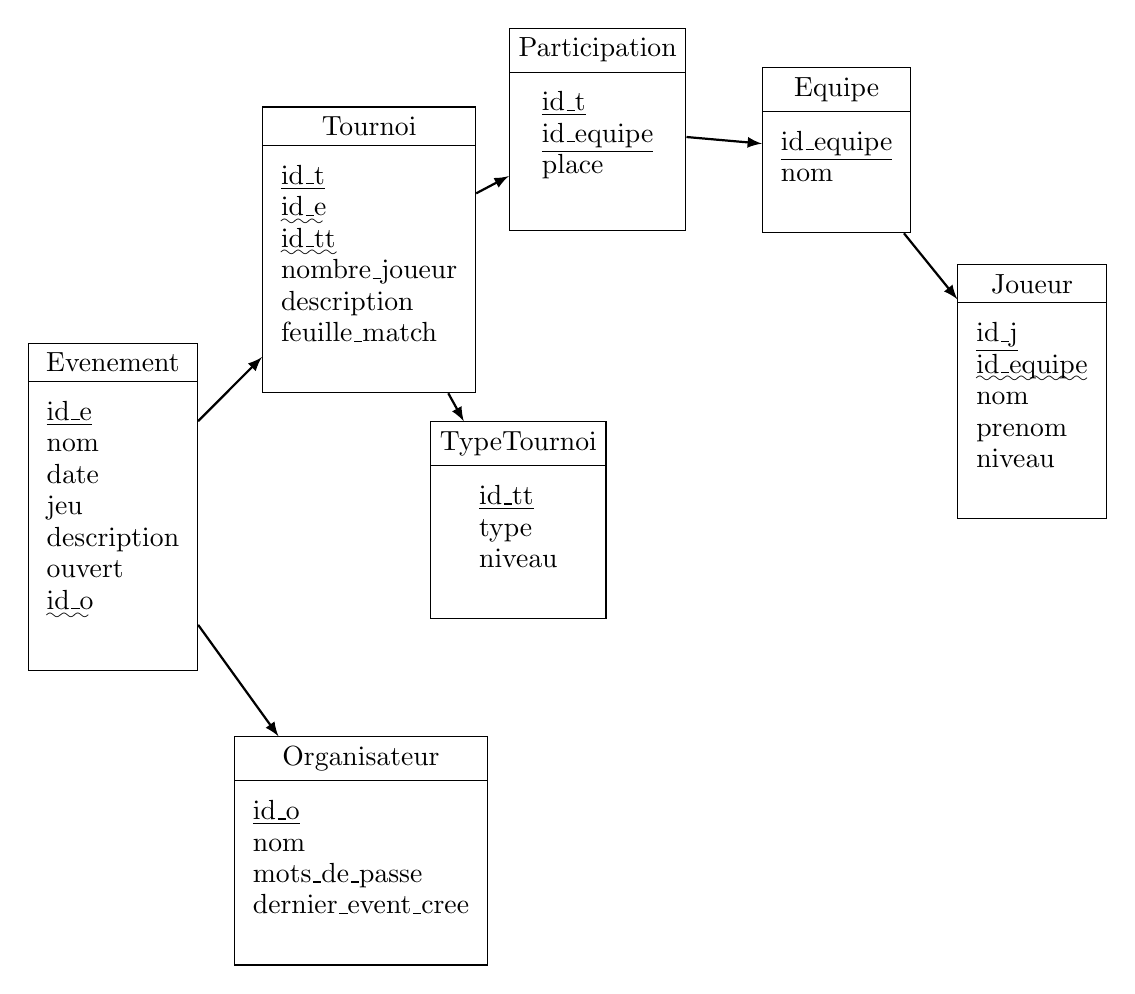
\begin{tikzpicture}[
					double/.style={draw, anchor=text, 		rectangle split, rectangle split parts=2},
					triple/.style={draw, anchor=text, rectangle split, rectangle split parts=3},
					triangle/.style={draw, shape=regular polygon, regular polygon sides=3,draw,thick,inner sep=0pt, minimum size=1cm, inner sep=-1.2cm, outer sep=0pt}]
					
    % Place nodes
    \node [double] (A) at (-6,0){Evenement
    	\nodepart{second}
    	\tikz{
    	\node at (0,0) {\underline{id\_e}};
    	\node at (0,-0.4) {nom};
    	\node at (0,-0.8) {date};
    	\node at (0,-1.2) {jeu};
    	\node at (0,-1.6) {description};
    	\node at (0,-2) {ouvert};
    	\node at (0,-2.4) {\uwave{id\_o}};
    }};
    \node [double] (B) at (0,4){Participation
    	\nodepart{second}
    	\tikz{
    	\node at (0,0) {\underline{id\_t}};
    	\node at (0,-0.4) {\underline{id\_equipe}};
    	\node at (0,-0.8) {place};
    }};
    \node [double] (C) at (-2.5,3){Tournoi
    	\nodepart{second}
    	\tikz{
    	\node at (0,0) {\underline{id\_t}};
    	\node at (0,-0.4) {\uwave{id\_e}};
    	\node at (0,-0.8) {\uwave{id\_tt}};
    	\node at (0,-1.2) {nombre\_joueur};
    	\node at (0,-1.6) {description};
    	\node at (0,-2) {feuille\_match};
    }};
    \node [double] (E) at (-3,-5){Organisateur
    	\nodepart{second}
    	\tikz{
    	\node at (0,0){\underline{id\_o}};
    	\node at (0,-0.4){nom};
    	\node at (0,-0.8){mots\_de\_passe};
    	\node at (0,-1.2){dernier\_event\_cree};
    }};
    \node [double] (F) at (3.5,3.5){Equipe
    	\nodepart{second}
    	\tikz{
		\node at (0,0) {\underline{id\_equipe}};
    	\node at (0,-0.4) {nom};
    }};
    \node [double] (G) at (-1,-1){TypeTournoi
    	\nodepart{second}
    	\tikz{
		\node at (0,0) {\underline{id\_tt}};
    	\node at (0,-0.4) {type};	 
    	\node at (0,-0.8) {niveau};	   	
    }};
    \node [double] (H) at (6,1){Joueur
    	\nodepart{second}
    	\tikz{
		\node at (0,0) {\underline{id\_j}};
		\node at (0,-0.4) {\uwave{id\_equipe}};
    	\node at (0,-0.8) {nom};	    	
    	\node at (0,-1.2) {prenom};	    
    	\node at (0,-1.6) {niveau};		
    }};
    \draw[thick,-latex] (A) edge (C);
    \draw[thick,-latex] (A) edge (E);
	\draw[thick,-latex] (C) edge (B);	
	\draw[thick,-latex] (C) edge (G);
	\draw[thick,-latex] (B) edge (F);
	\draw[thick,-latex] (F) edge (H);	
    % Draw edges
    
\end{tikzpicture}~\\

\end{figure}~\\
\newpage

{\textbf{\Large Modelé Relationnelle}\\

evenement(\underline{id\_e}, nom, date, jeu, description, ouvert, \uwave{id\_o})

participation(\underline{id\_equipe},\underline{id\_t}, place)

tournoi(\underline{id\_t}, \uwave{id\_tt}, \uwave{id\_e}, nombre\_joueur, description, feuille\_match)

typetournoi(\underline{id\_tt}, type, niveau)

equipe(\underline{id\_equipe}, nom)

joueur(\underline{id\_j}, \uwave{id\_equipe}, nom, prenom, niveau)

organisateur(\underline{id\_o} , nom, mot\_de\_passe, dernier\_event\_cree)


\end{document}